%----------------------------------------------------------------------------
\chapter{Megvalósítás}
%----------------------------------------------------------------------------
\section{Szükséges eszközök}
\subsection{Eclipse}
A feladatot Eclipse-be integrált tervezőeszközként valósítottam meg. Ez egy szabadon bővíthető nyílt forráskódú szoftverkeretrendszer. Sokféle modellező eszköz integrálható  Eclipse-be. Azért ezt választottam mert a modellezés általam használt részeihez is biztosít megfelelő keretrendszereket.
\subsection{Metamodell}
A metamodell összefoglalja egy modellezési nyelv legfőbb fogalmait, relációit és alapvető struktúráját. Egy olyan alapséma, amire illeszkedik az összes hozzá tartozó alacsonyabb absztrakciós szinttel rendelkező modell. 
Tegyük fel hogy M* modell M1 modellnek a metamodellje.
Akkor M* metamodell meghatározza az M1 modellben lévő elemeket, attribútumokat és ezeknek lehetséges kapcsolatait. Például az alábbi modelleknek (lásd \autoref{jarmupeldany}) a már korábban említett jármű modell (lásd \autoref{jarmu}) tekinthető metamodelljének. Bal oldalon egy motor példánymodellje, jobb oldalon pedig egy biciklinek a modellje látható.

\begin{figure}[!ht]
	\centering
	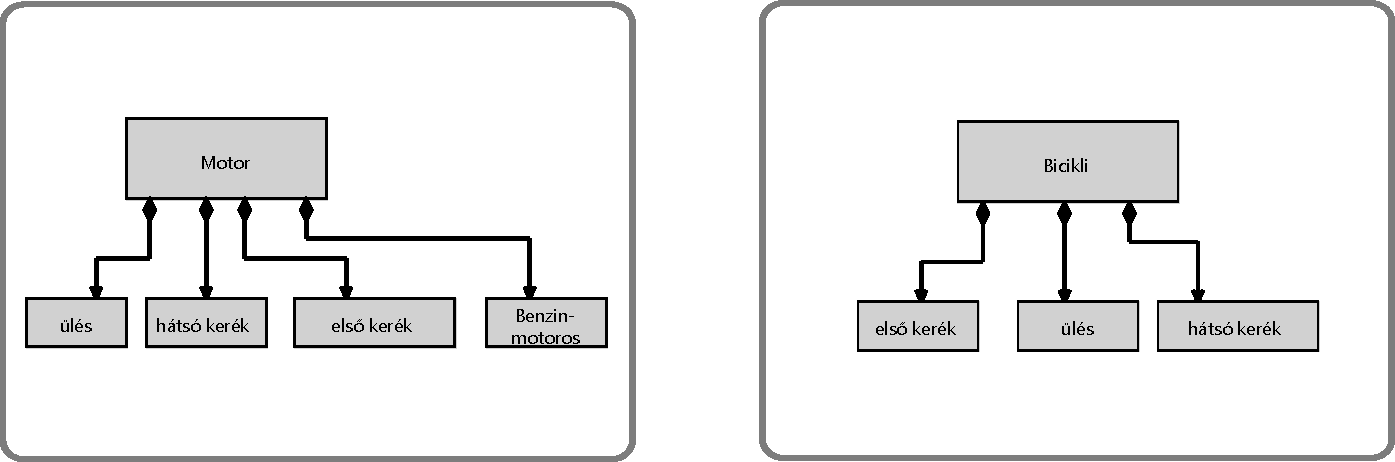
\includegraphics[width=130mm]{figures/peldany.pdf}
	\caption{Jármű metamodellhez tartozó példánymodellek} 
	\label{jarmupeldany}
\end{figure}

\subsection{EMF}
\nocite{EMFtut}
EMF az Eclipse Modelling Framework \cite{EMF} rövidítése. Ez egy olyan keretrendszer, mely az eclips-be beépülve teszi lehetővé modellek készítését. Segítségével könnyedén grafikus eszközökkel lehet metamodelleket alkotni, melyből később konkrét példánymodellt készíthetünk. Továbbá lehetőséget biztosít metamodellből java kódot generálni, ami leképezi a modell elemeit osztályokba és a hozzá tartozó kapcsolatokat és attribútumokat is.

\subsection{Sirius}
\nocite{SiruisTutNagyASz}
\nocite{SiruisTutStart}
\nocite{SiruisTutAdv}
Ez egy szintén Eclipse-be épülő keretrendszer \cite{Sirius}. Ez lehetővé teszi hogy EMF modellekhez vizuális megjelenítő és szerkesztő felületet készítsünk. Rendkívül sokrétű lehetőséget nyújt. Lehetőség van új objektumok létrehozására szerkesztésére és biztosít validációs lehetőségeket is. Az egyes elemek módosítását megszorításokhoz lehet kötni. Egy úgynevezett "viewpoint specification" projektet kell létrehozni, majd ezen belül egy "odesign" kiterjesztésű fájlt. Ebben a fájlban be kell állítani milyen modellel szeretnénk dolgozni és azután lehet a modellhez tartozó editor működését és megjelenését definiálni. Ki lehet választani milyen típusú reprezentációt szeretnék a modellemnek, például: diagram, táblázat, fastruktúra. Meg lehet adni hogy a modellben lévő elemek vizuálisan hogyan jelenjenek meg. Ez a stílus akár dinamikusan változhat az elem tulajdonságától függően. Ebben a fájlban lehet pontosan megadni, hogy mi történjen egy elem létrehozásánál, törlésénél vagy módosításánál. Ezen események bekövetkezése kiválthatnak további eseményeket, ezáltal láncba fűzhetők. Például kitörlök egy elemet és ennek következtében módosítok egy másikat. A Sirius-szal lehet elágazásokat definiálni (switch-case, if) és iterációt is támogat (for ciklus). Sirius képes külső Java kód futtatására, amivel bővíthető a szerkesztőfelület funkcionalitása.

\subsection{Java}
Objektumorientált programozási nyelv. EMF keretrendszer lehetőséget biztosít arra, hogy az elkészített modellből Java kód generálható. Az EMF modellből kigenerált kódot futtatva egy új Eclipse alkalmazás indítható, melyben már lehetőség van a metamodellben definiált modell példányosítására. 

\subsection{Aql}
\nocite{Acceleo}
\nocite{OCL}
Az Annotation Query Language \cite{Aql} rövidítése. Lambda \cite{Lambda} kifejezésekhez hasonlóan lehet alkalmazni. 
%A lambda kifejezés egy névtelen függvény, ami 
Az editor elkészítésébe van nagy szerepe. Az egyes funkciókat előfeltételeit lehet leírni ezen a nyelven. 

%\section{Metamodell szerkezete}

\subsection{Általános modell}

\subsubsection{Jellemzés}
Egy általános modell elemekből áll, amik tulajdonságokkal rendelkeznek, az elemek között pedig kapcsolatok vannak. Tehát olyan meta modellt kell készíteni, ami mindezeket magába foglalja. A metamodell elkészítéséhez EMF-et használtam (lásd \autoref{model}).

\begin{figure}[!ht]
	\centering
	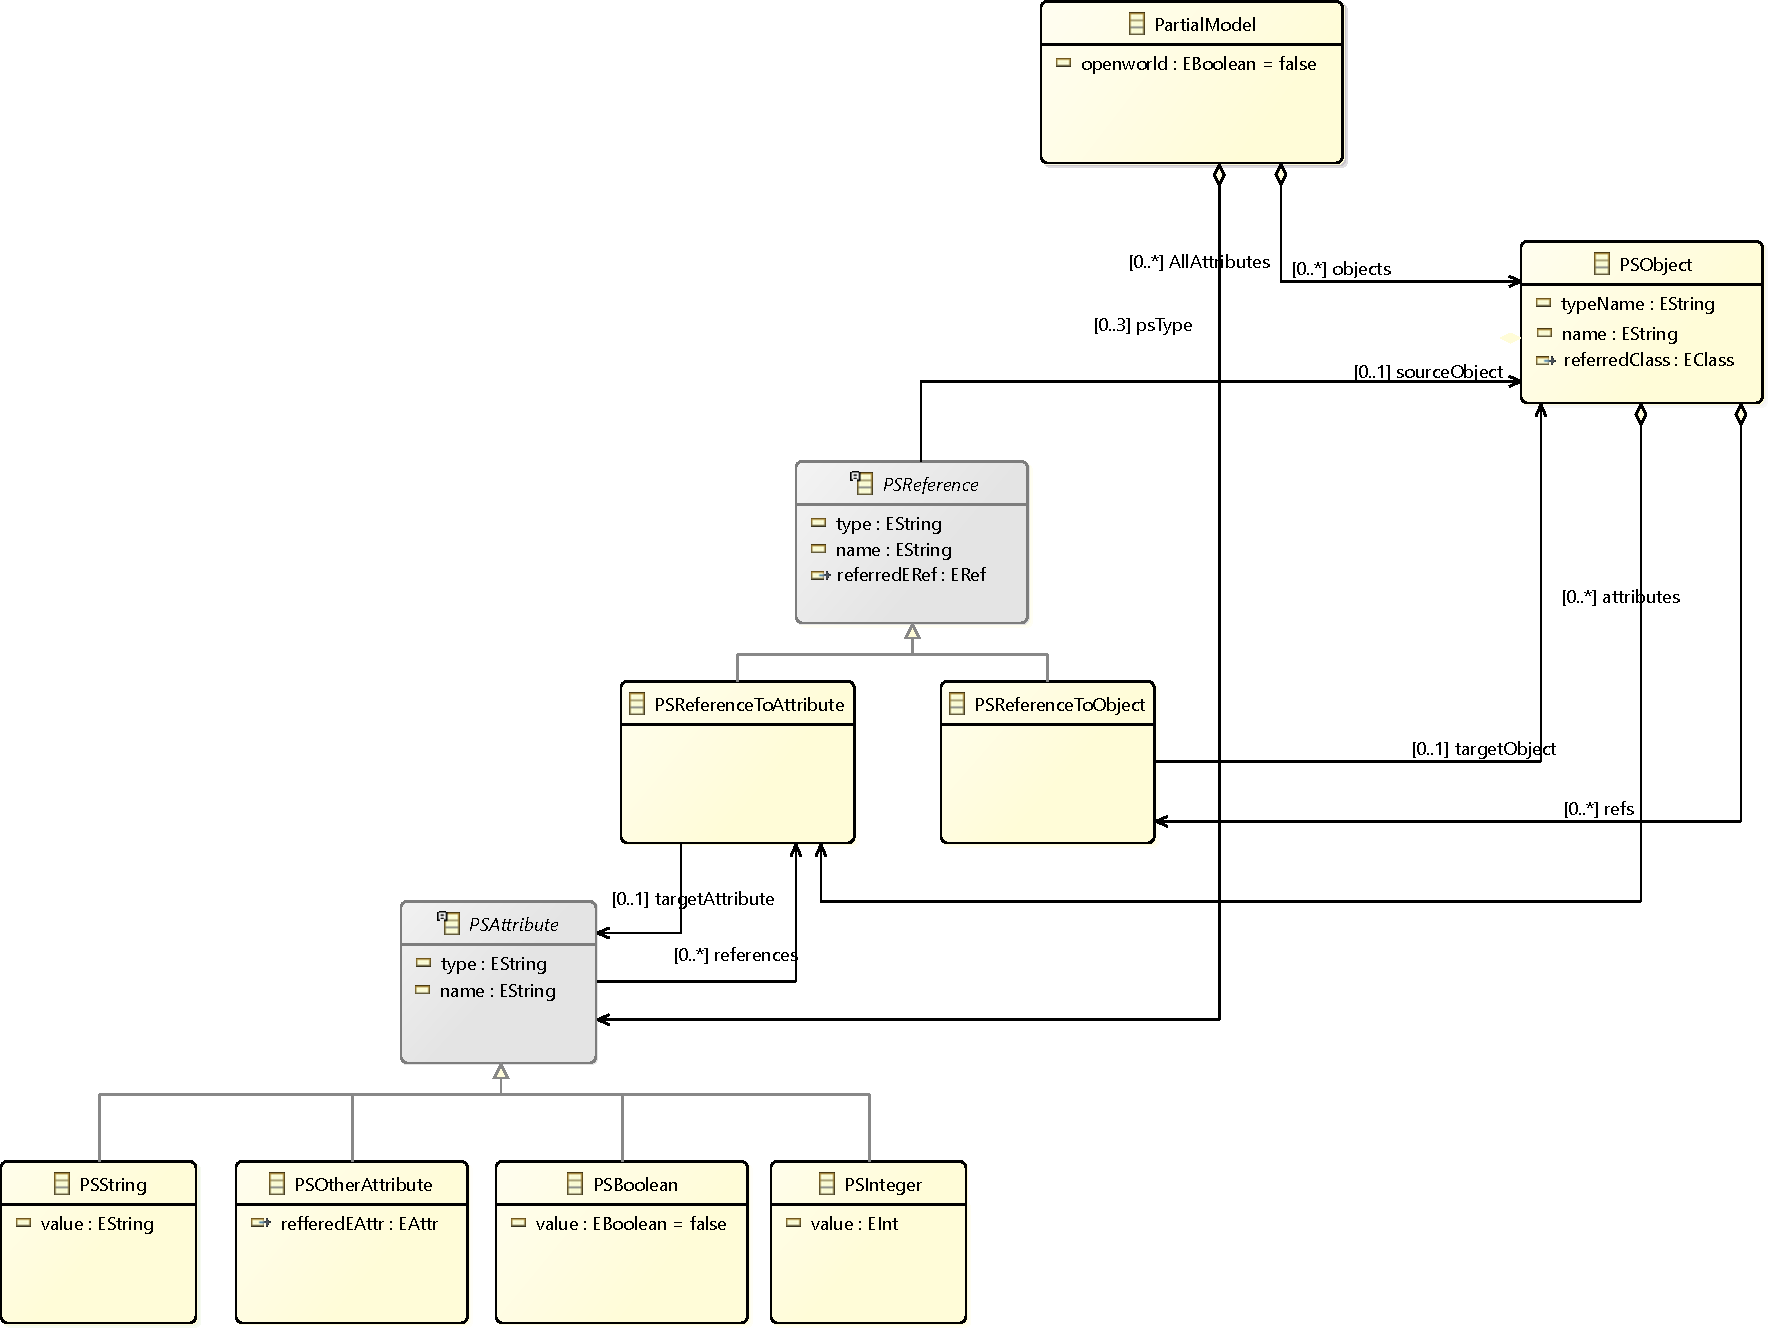
\includegraphics[width=150mm]{figures/partialmodel01.pdf}
	\caption{Általános modell, ami legtöbb modell metamodelljének tekinthető} 
	\label{model}
\end{figure}

\subsubsection{PSObject}
A modellben a PSObject-ek reprezentálják az általános modell elemeit. Ez bármilyen típusú lehet. Rendelkezik névvel (name), referált osztállyal (ReferredEClass) és a referált osztály konkrét példányának az azonosítójával (uri). így a PSObject-en keresztül tudunk részlegességet rendelni a hivatkozott objektumhoz, ami erre egyébként nem lenne képes. PSObjectek tartalmaznak tetszőleges mennyiségű referenciát másik objektumokra (PSReferenceToObject) és attribútumokra (PSReferenceToAttribute).

\subsubsection{PSReference}
 Az elemek közötti kapcsolatokat reprezentálják. Fontos, hogy ezek is külön elemként jelenjenek meg a modellben, hisz ehhez is szeretnénk majd részlegességet társítani annotációk formájában. A PSReference egy absztrakt objektum két leszármazottja van a  PSReferenceToAttribute és PSReferenceToObject. Erre azért volt szükség mert későbbiekben a szerkesztő elkészítésénél más funkcionalitások vonatkoznak rájuk és logikailag is kifejezi, hogy az attribútum valamelyik objektum része és csak azzal együtt érvényes, míg egy objektum önmagában is értelmezhető. Rendelkezik névvel (name), referált osztállyal (ReferredEClass) és típussal (type). Van neki forrásobjektuma (sourceObject) és célobjektuma (targetObject) vagy célattribútuma (targetAttribute).

\subsubsection{PSAttribute}
Az objektumok tulajdonságai külön egy PSAttribute nevű elemben vannak hozzárendelve az objektumokhoz, így lehetőség van az attribútumokhoz is részlegességet rendelni. Lehetséges továbbá az is hogy egy attribútum több objektumhoz is tartozzon, ugyanis az attribútumokat nem közvetlenül a PSObjeckt-ek tárolják hanem csak hivatkoznak rájuk. Azonban az attribútumok tárolják a rájuk mutató PSReference-ek referenciáit. PSAttribute is absztrakt ezért több fajtája lehet:

\begin{itemize}  
	\item PSString
	\item PSBoolean
	\item PSInteger
	\item PSOtherAttribute 
\end{itemize}


\subsection{Kiegészítés részleges modellé}

\subsubsection{OW részlegesség}
Az \textit{OW} részlegességet a modell gyökerében egy boolean változóval tudjuk szemléltetni.

\subsubsection{PSType}
Minden egyes modellbeli elemhez tudnunk kell társítani annotációkat. Ezt a PSType-al tehetjük meg (lásd \autoref{partialmodel}), amiből leszármaznak a már említett részlegesség fajták (\textit{May}, \textit{Var}, \textit{Abs}):

\begin{itemize}  
	\item MayType
	\item AbsType
	\item VarType 
\end{itemize}

\begin{figure}[!ht]
	\centering
	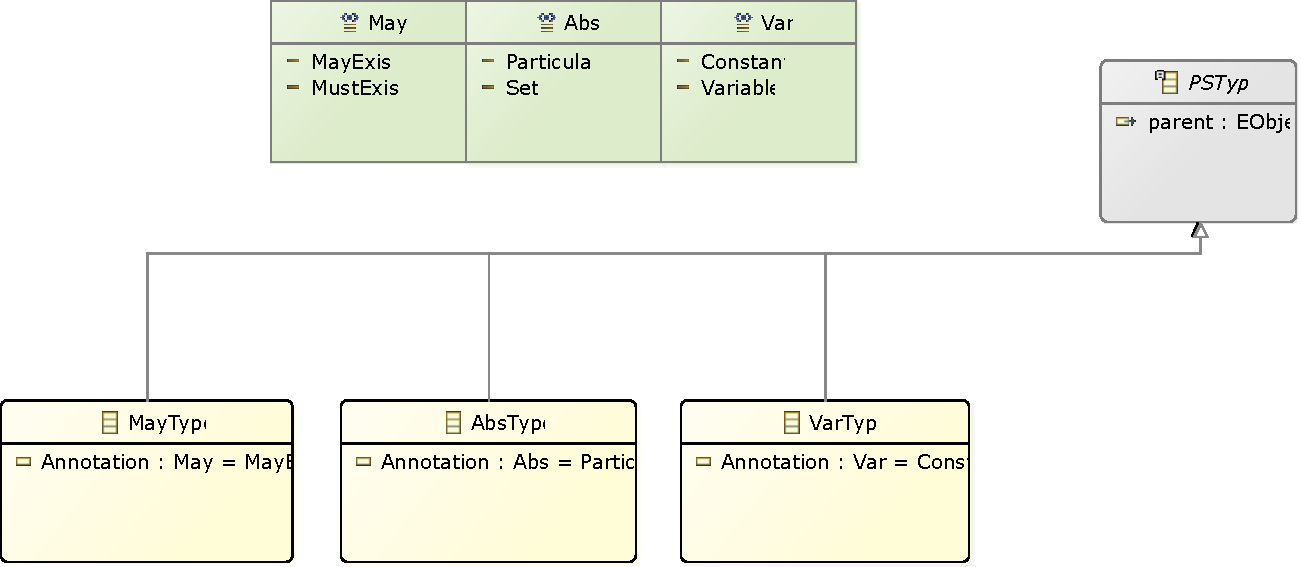
\includegraphics[width=150mm]{figures/partialmodel02.pdf}
	\caption{Általános modell kiegészítve részleges modellekre jellemző tulajdonságokkal}
	\label{partialmodel} 
\end{figure}

\section{Szerkesztő}
\subsection{Példánymodell felülete}
\subsubsection{PSObject}
Világoszöld téglalapként jelenik meg (lásd \autoref{obj}).  A téglalap fejrészében megjelenik az objektum neve.
\begin{figure}[!ht]
	\centering
	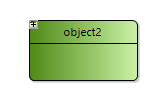
\includegraphics{figures/obj.PNG}
	\caption{PSObject}
	\label{obj} 
\end{figure}
\\\\
Funkciók:
\begin{itemize}  	
	\item Bal felső sarkában pedig egy kis '+' jel segítségével megjeleníthetjük a hozzá tartozó attribútumokat. Amennyiben ezek láthatóak akkor egy '-' jel jelenik meg amivel elrejthetjük. 	
	
	\item PSObject létrehozása a szerkesztőfelület oldalán lévő sávból kiválasztva lehetséges. Az Object nevet kiválasztva, majd a szerkesztőfelületre kattintva megjelenik a négyzet egy alapértelmezett névvel. A név formátuma: 'Object\{szám\}'. A szám helyén egy automatikusan generált szám kerül, a már meglévő PSObject-ek száma növelve eggyel. Ezt aql kifejezéssel lehet megtenni: 
	\begin{align}
	aql:'object'+container.objects->size()
	\end{align}	

	\item Az objektum nevére rákattintva az közvetlenül szerkeszthetővé válik. A többi tulajdonság a Sirius által alapból biztosított 'Properties' fülön érhető el. 
	
	\item Törlés esetén megsemmisül az objektumból kivezető összes referencia. Sirius tartalmazás esetén automatikusan kitörli az objektumban lévő egyéb elemeket. Az objektumra mutató referenciák viszont nem törlődnek maguktól, mert a forrás PSObject-ben vannak. Mivel a PSObject nem tárolja a rá mutató éleket így először az összes PSObject referenciáján végigiterálva kitörli azokat, amik rá mutatnak, majd törli önmagát is. 
\end{itemize}


\subsubsection{PSReference}
A felületen szürke vonalként jelenik meg. Összeköthet PSObject-et attribútummal vagy egy másik PSObject-el. Utóbbi esetben a vonal végén nyíl is van. A referencián szövegesen megjelenik neve és zárójelben a hozzá tartozó részlegességek is. Amennyiben rákattintunk a referenciára kétszer megjelenik egy másik szerkesztőfelület, ahol a referencia egy narancssárga téglalapként jelenik meg (lásd \autoref{ref}).
\begin{figure}[!ht]
	\centering
	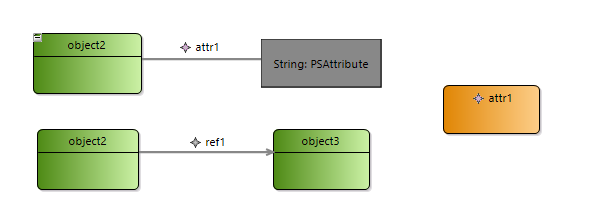
\includegraphics{figures/ref.PNG}
	\caption{PSReference (baloldalt a részleges modellen megjelenő formában, jobb oldalon a rákattintás utáni nézet látható)}
	\label{ref} 
\end{figure}
\\\\
Funkciók:
\begin{itemize}  	
	\item Kétszer rákattintva egy referenciára megjelenik egy új szerkesztőfelület. Itt csak egy narancssárga téglalap van a referencia nevével. Erre a nézetre azért van szükség, mert részlegességek így könnyebben kezelhetők. A részlegességek magyarázatánál bővebben lesz erről szó.
	
	\item Létrehozása a szerkesztőfelület oldalán lévő sávból kiválasztva lehetséges (reference). Aztán egy PSObject-re kattintva a kezdőpontja, majd második kattintásra a cél objektuma vagy attribútuma jelölhető ki a referenciának. A kiválasztó felületen nincs külön referencia objektumra és attribútumra, ez a felhasználó számára rejtve marad, azonban a háttérben mégis külön kezelődik. Referencia létrehozásának a logikájában van egy elágazás (switch), ami vizsgálja, hogy a célobjektum, tehát amire másodjára kattintunk az milyen típusú. A referencia típusát aql kifejezéssel lehet eldönteni (lásd \autoref{refcreation}). A referencia nevét hasonlóan a PSObject-hez aql segítségével generálja: 'attr\{szám\}' vagy 'ref\{szám\}'. Itt a 'szám' a forrás objektumból kiinduló attribútumokra vagy objektumokra mutató referenciák számát veszi figyelembe. Attribútumra mutató referencia esetében kicsit különbözik a működés. Amennyiben a referált attribútumra már mutat másik referencia, akkor az új referenciához automatikusan hozzá generálunk egy May részlegességet. Ennek az az értelme, hogy gyakorlatban nem fordulhat elő olyan, hogy egy attribútum több objektumhoz is tartozik.
	
	\item Éleket át lehet huzalozni, azaz másik célelemet lehet választani nekik. PSObject-re mutató élt nem lehet megváltoztatni PSAttribute-ra mutató élre és fordítva se. Új cél kiválasztása esetén a régi felülíródik. Attribútum esetében a régi attribútumból törlődik az él referenciája és az új attribútumba íródik be. Ha attribútumról olyan attribútumra húzzuk át az élet, amibe már vezet él akkor ahhoz  automatikusan hozzá generálódik egy 'May' részlegesség, mint ahogy az új él létrehozásnál is történt.
	
	\item Törlés esetén nem szükséges plusz logikát beiktatni. Sirius  beépítetten kezeli.
\end{itemize}

\begin{figure}[!htp]
	\centering
	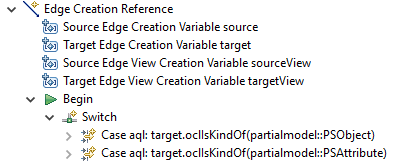
\includegraphics[width=100mm]{figures/refcreation.PNG}
	\caption{Referencia létrehozásának logikája}
	\label{refcreation} 
\end{figure}

\subsubsection{PSAttribute}
Szürke téglalapként jelenik meg a szerkesztőfelületen (lásd \autoref{attr}). Az attribútum típusa és értéke a téglalap közepén látható kettősponttal elválasztva.
\begin{figure}[!ht]
	\centering
	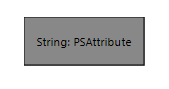
\includegraphics{figures/attr.PNG}
	\caption{PSAttribute}
	\label{attr} 
\end{figure}
\\\\
Funkciók:
\begin{itemize}  	
	\item Létrehozása a szerkesztőfelület oldalán lévő sávból kiválasztva lehetséges (UndefinedAttribute). Ezután a szerkesztő panelen kattintva létrejön egy attribútum. Ez nem tartozik még egyetlen objektumhoz sem.
	
	\item A típusának és értékének szerkesztése lehetséges a Sirius által biztosított 'Properties' fülön.
	
	\item Törlésénél végig iterál az összes rá mutató referencián és kitörli azokat, majd törli önmagát is.	

\end{itemize}

\subsubsection{PSType}
A szerkesztőfelületen világoszöld téglalapként jelenik meg az elem mellett, amihez hozzá lett rendelve (lásd \autoref{part}). Referencia esetén zárójelben látszik az él neve előtt, de ha kétszer rákattintunk a referenciára, hogy megnyissuk a szerkesztőfelületét, ott az élet reprezentáló narancssárga téglalap mellett fog megjelenni (lásd \autoref{obj}).
\begin{figure}[!ht]
	\centering
	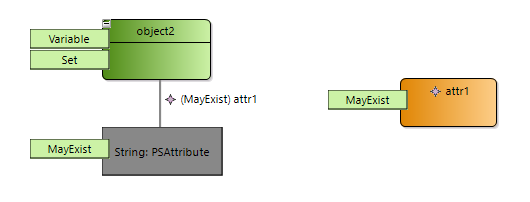
\includegraphics{figures/part.png}
	\caption{PSType (baloldalt a részleges modell szerkesztőfelülete, jobb oldalon a referencia szerkesztőfelülete)}
	\label{part} 
\end{figure}
\\\\
Általános funkciók:
\begin{itemize}  	
	\item Létrehozása a szerkesztőfelület oldalán lévő sávból kiválasztva lehetséges (May, Abs, Var), utána arra az elemre kattintva amelyikhez a részlegességet hozzá akarom rendelni létrejön a PSType. Él esetében ugyan ez a referencia saját szerkesztőfelületén lehetséges.
	
	\item Törlés esetén nem szükséges plusz logikát beiktatni. Sirius  beépítetten kezeli.	
\end{itemize}

\subsection{Finomítás}
Duplán kattintva a PSType-ra történik meg a feloldása a részlegességnek. A PSType-nak három fajtája van, amik különböző módokon viselkednek attól függően, hogy milyen típusú elemre vannak rátéve, ezért ezeket külön tárgyalom. 

\subsubsection{PSObject May feloldása}
Feloldásnál az objektum és az összes hozzátartozó attribútum törlődik. Ezt úgy oldottam meg, hogy végigiterál az összes élen ami attribútumra mutat és törli azokat. Amennyiben az attribútumra mutat más objektumból is referencia akkor az nem törlődik (lásd \autoref{objmay}).
Aql feltétel, ami azt vizsgálja, hogy nem vezet-e más objektumból él az attribútumba:
\begin{align}
 aql:ref.targetAttribute.references->forAll(x | x.sourceObject = element.eContainer())
\end{align}
\begin{figure}[!ht]
	\centering
	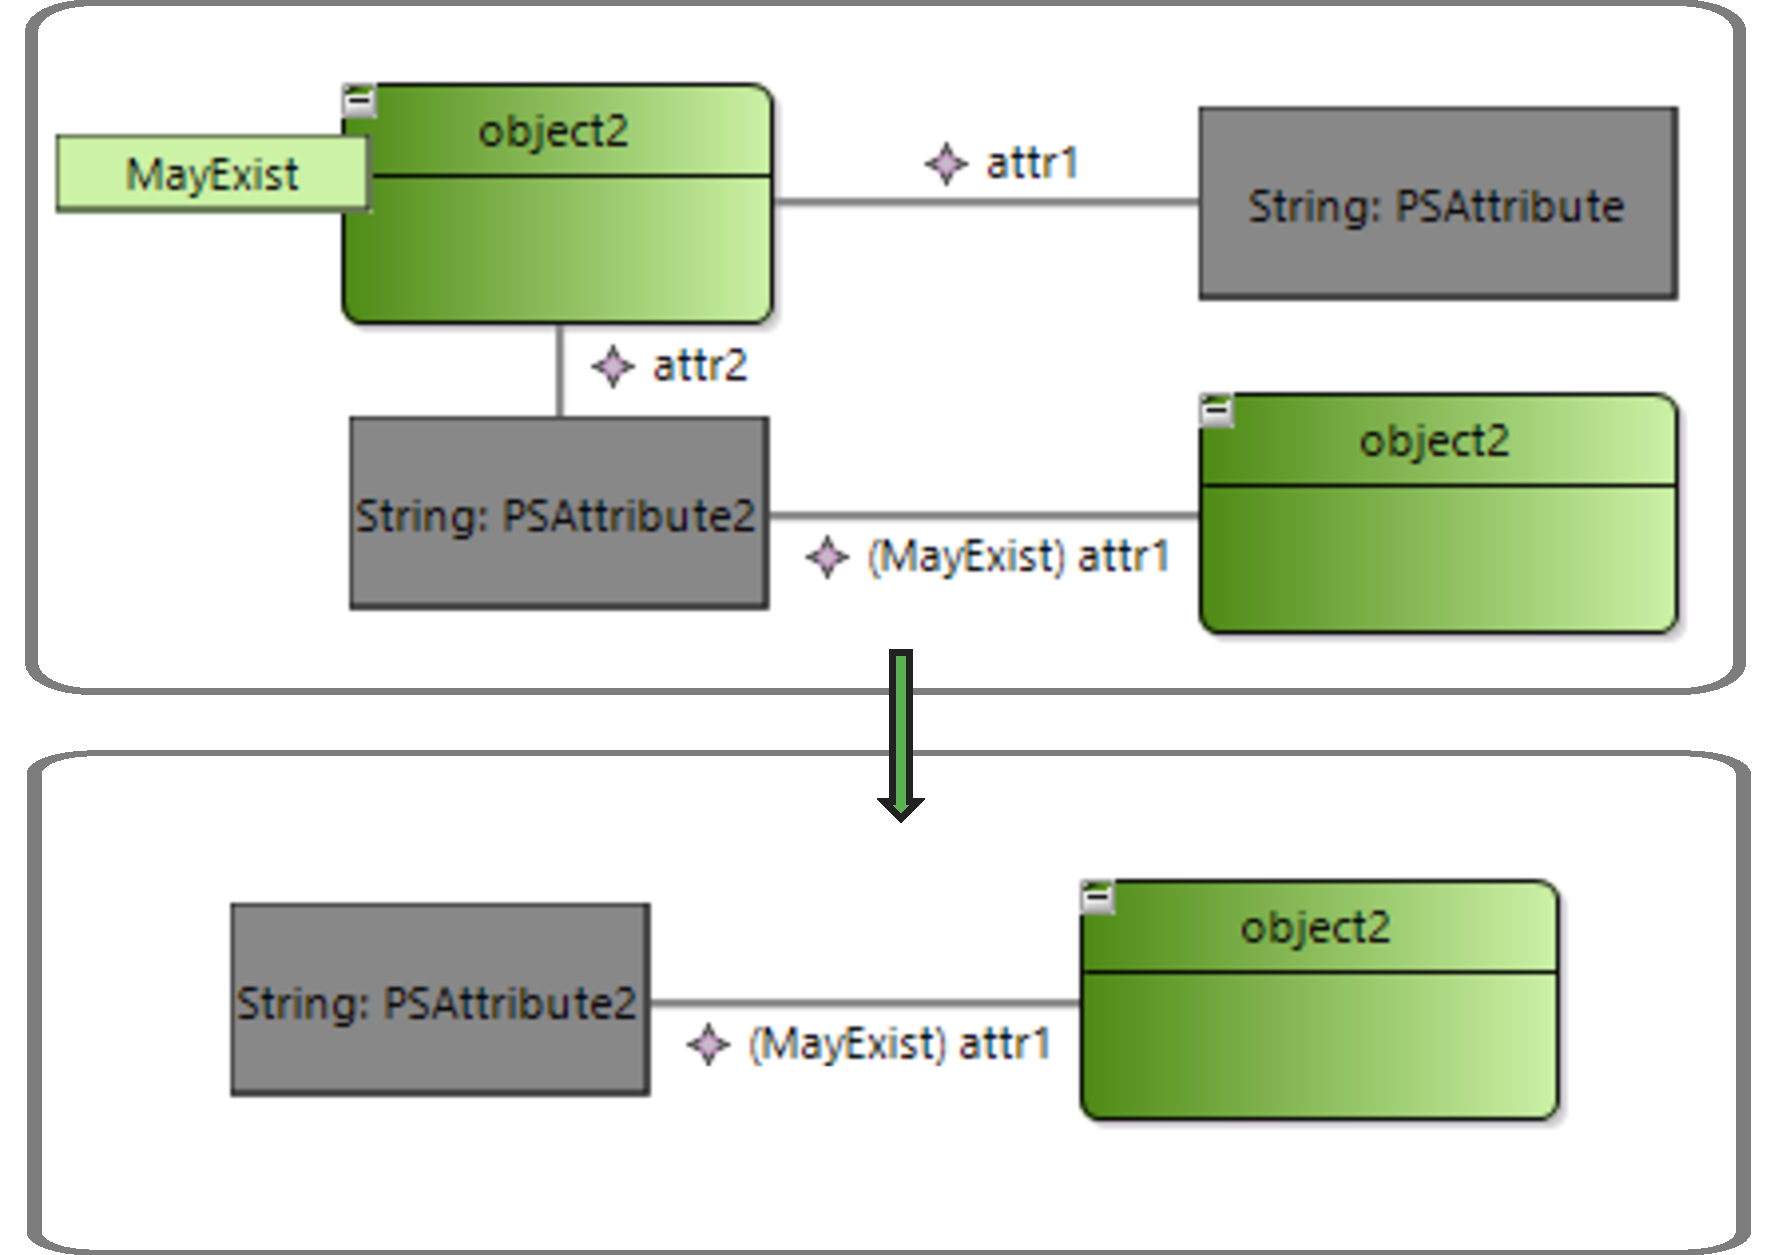
\includegraphics[width=100mm]{figures/objmay.pdf}
	\caption{PSObject finomítása (May)}
	\label{objmay} 
\end{figure}

\subsubsection{PSAttribute May feloldása}
Élek nem törlődnek automatikusan mert a PSObject tartalmazza őket. Végig kell iterálni az összes attribútumra mutató élen és kitörölni azokat. Ezután kitörlődik az attribútum is (lásd \autoref{attrmay}). 
\begin{figure}[!ht]
	\centering
	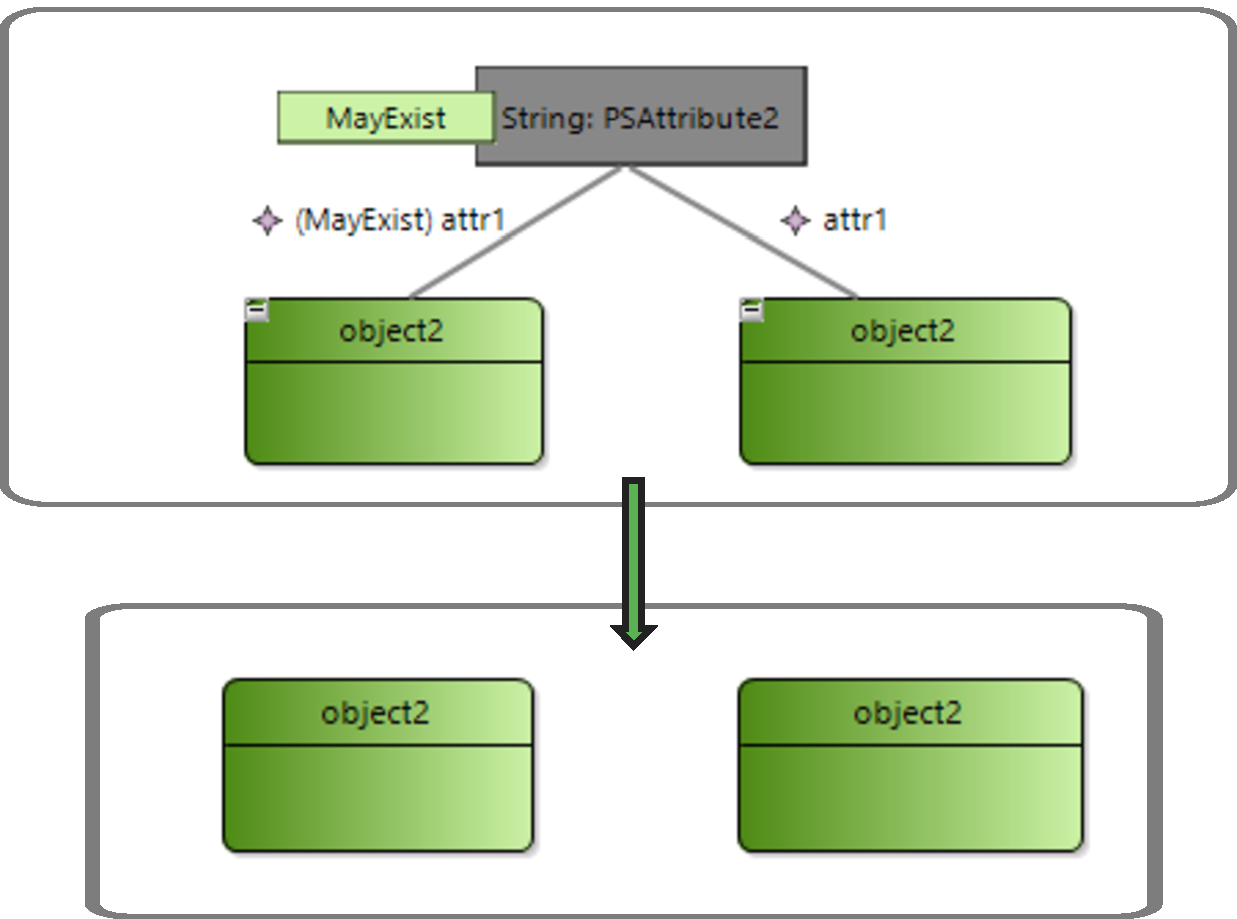
\includegraphics[width=100mm]{figures/attrmay.pdf}
	\caption{PSAttribute finomítása (May)}
	\label{attrmay} 
\end{figure}

\subsubsection{PSReferenceToObject May feloldása}
Kitörli a referenciát a forrásobjektumból.

\subsubsection{PSReferenceToAttribute May feloldása}
Az él törlődik, de eltérően az PSObject-ekre mutató referenciától, amennyiben a célattribútumba nem vezet másik él, akkor az attribútum is megszűnik. A finomítás lényege, hogy általa csökken a részlegessége a modellnek. Ezért nem lenne értelme az üresen maradt attribútumot meghagyni, ami nem kötődik semmilyen objektumhoz, mert nem csökkent volna a modell részlegessége (lásd \autoref{refmay}).
\begin{figure}[!ht]
	\centering
	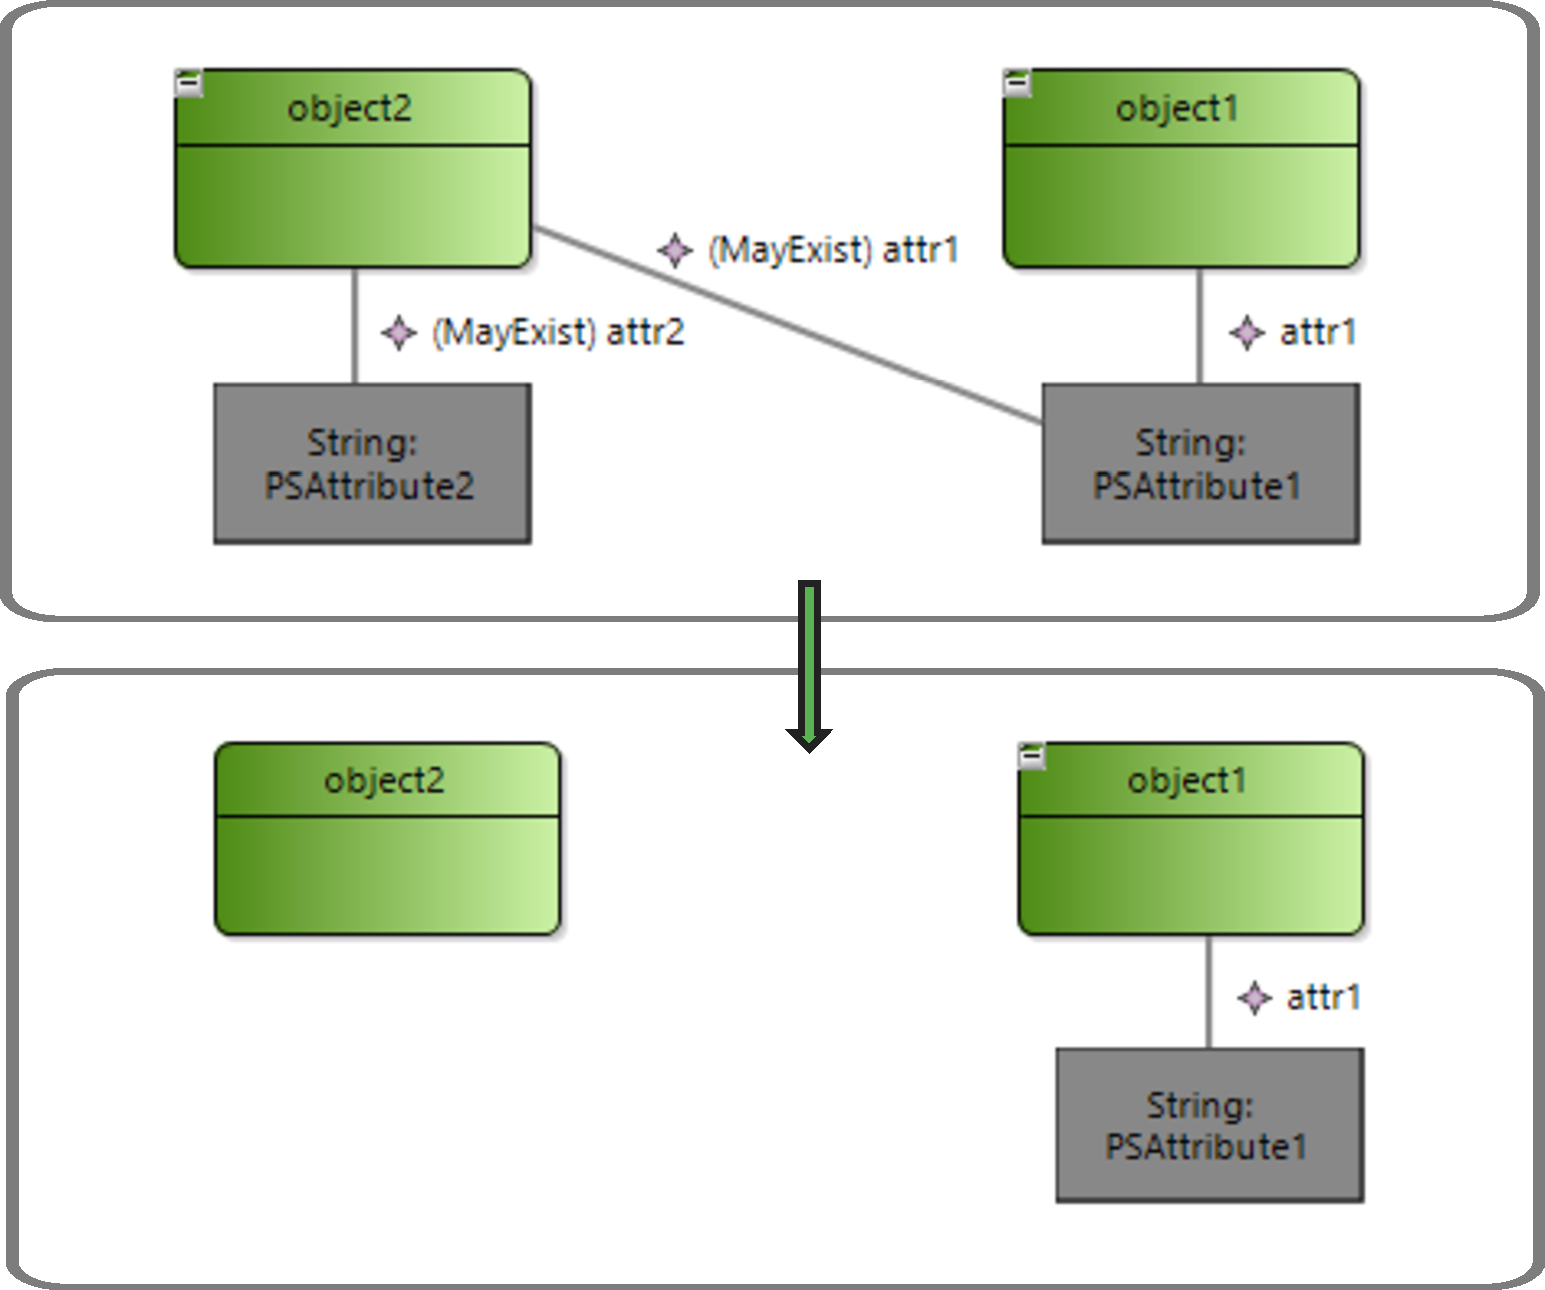
\includegraphics[width=100mm]{figures/refmay.pdf}
	\caption{PSReferenceToAttribute finomítása (May)}
	\label{refmay} 
\end{figure}

\subsubsection{PSObject Set feloldása}
Létrejön egy új objektum, aminek ugyanazok a tulajdonságai, mint az eredeti objektumnak, amin a 'Set' annotáció volt. Az új PSObject referenciái ugyan azokra az objektumokra mutatnak, mint az eredeti PSObject-nél. Új attribútumok jönnek létre az eredeti objektumhoz tartozó attribútumok mintájára és ezek lesznek az új elem attribútumai. Az új élek nevei ugyan azok mint az eredetié de a végére kerül egy kis 'v' betű (lásd \autoref{objset}).
\begin{figure}[!ht]
	\centering
	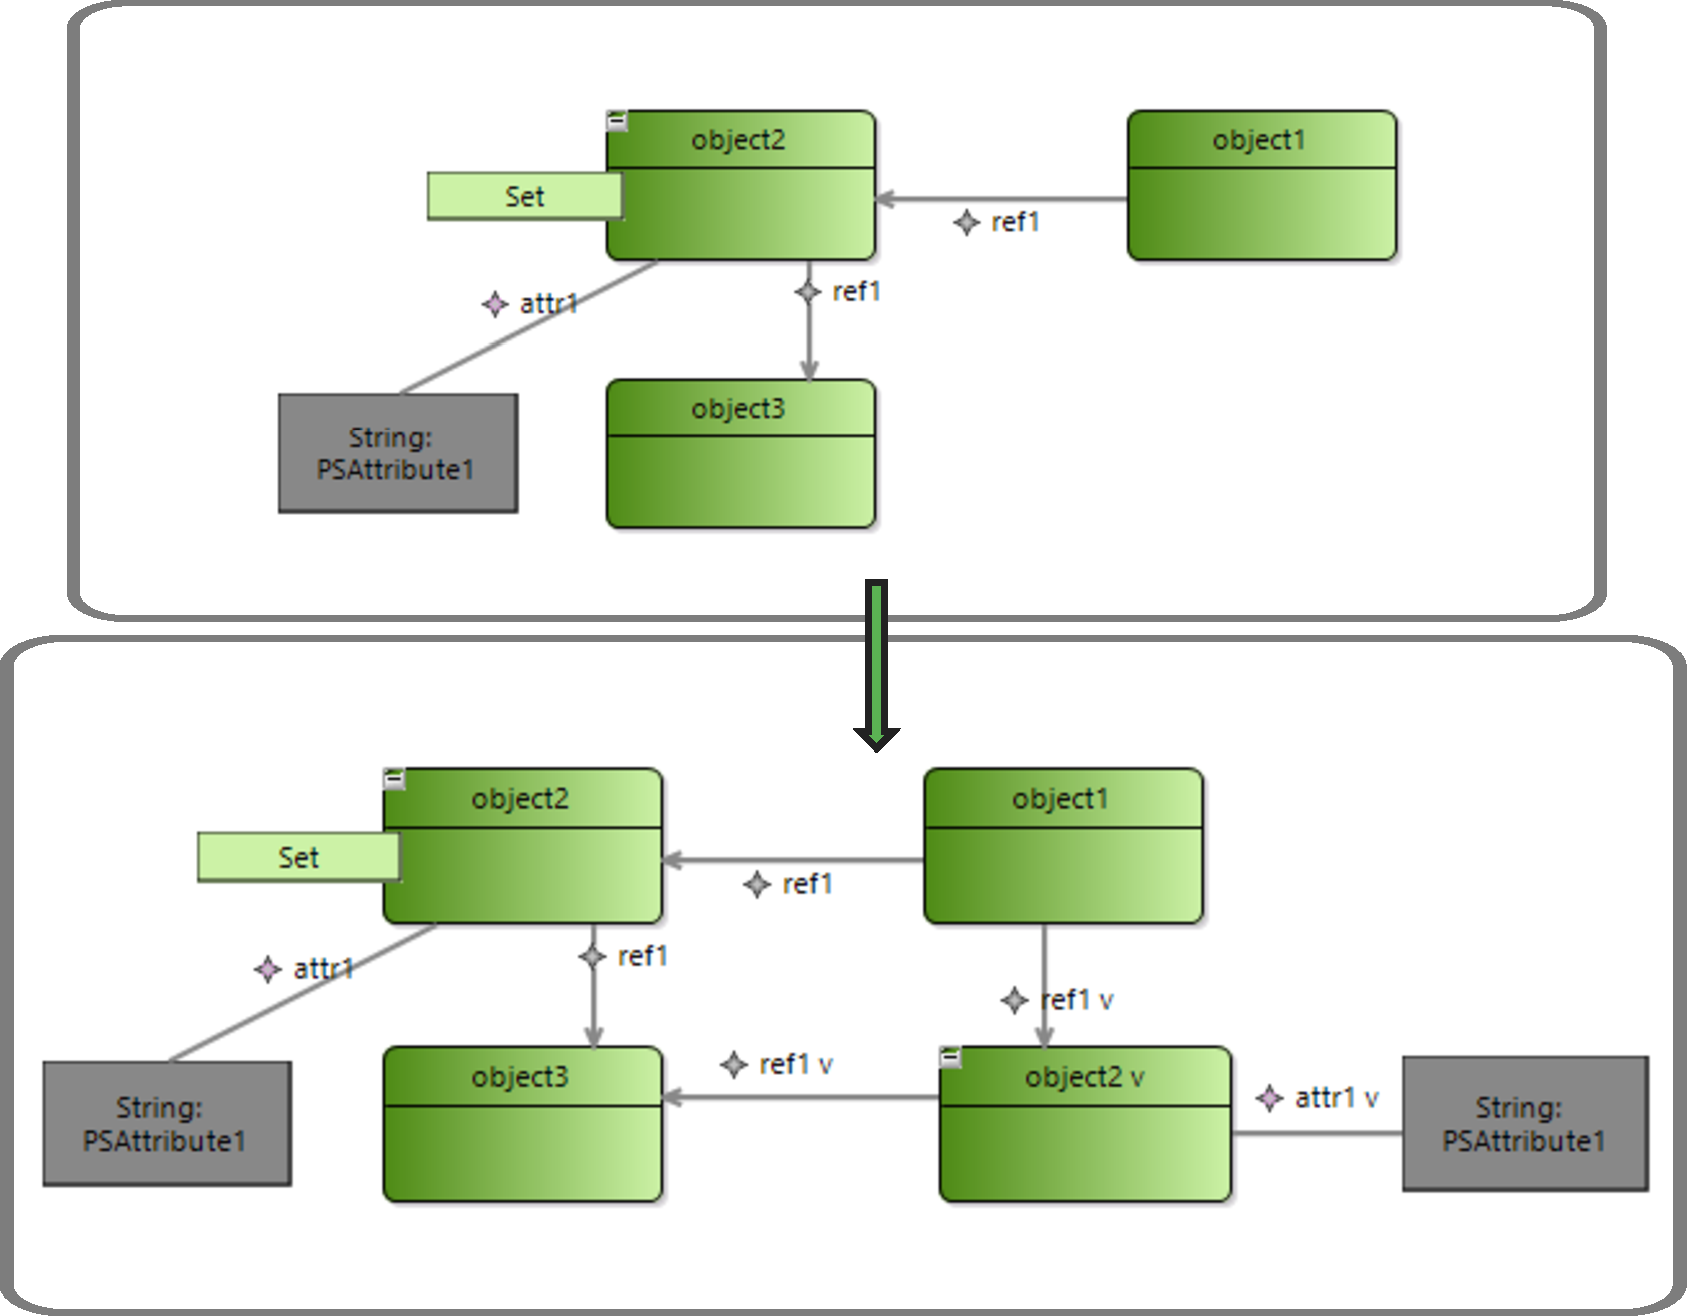
\includegraphics[width=100mm]{figures/objset.pdf}
	\caption{PSObject finomítása (Set)}
	\label{objset} 
\end{figure}

\subsubsection{PSAttribute Set feloldása}
Létrejön egy új attribútum és ugyan ahhoz az PSObject-hez fog tartozni mint az eredeti. Tehát az objektumból él fog vezetni az attribútumba. A típusát és értékét is megörökli az eredeti attribútumnak. Új elemhez tartozó referenciák nevei után egy kis 'v' betű kerül (lásd \autoref{attrset}).
\begin{figure}[!ht]
	\centering
	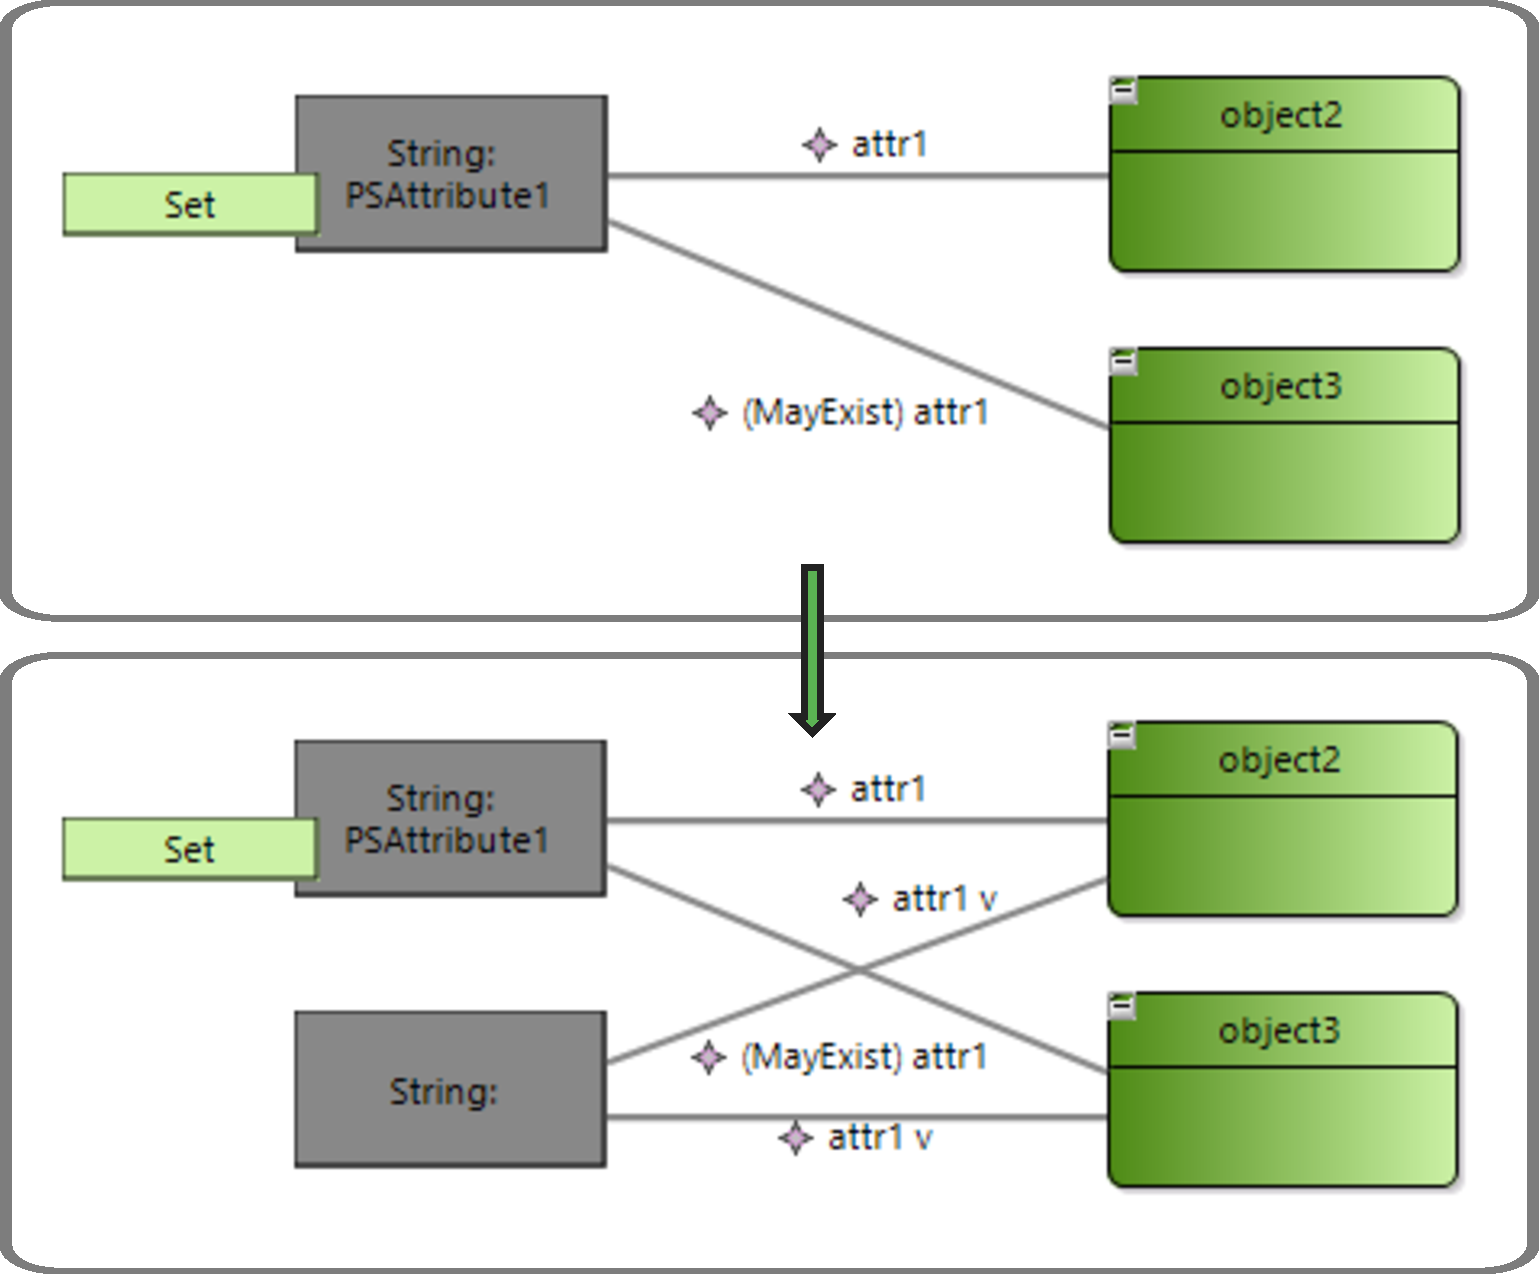
\includegraphics[width=100mm]{figures/attrset.pdf}
	\caption{PSAttribute finomítása (Set)}
	\label{attrset} 
\end{figure}

\subsubsection{PSReferenceToObject Set feloldása}
Az eredeti referencia forrásobjektumában létrehoz egy újat, ami ugyan arra az objektumra mutat (lásd \autoref{refset}).

\subsubsection{PSReferenceToAttribute Set feloldása}
Az eredeti referencia forrásobjektumában létrehoz egy újat, ami ugyan arra az attribútumra mutat, ezután a célattribútum referenciái közé is hozzáadjuk az új élet(lásd \autoref{refset}).
\begin{figure}[!ht]
	\centering
	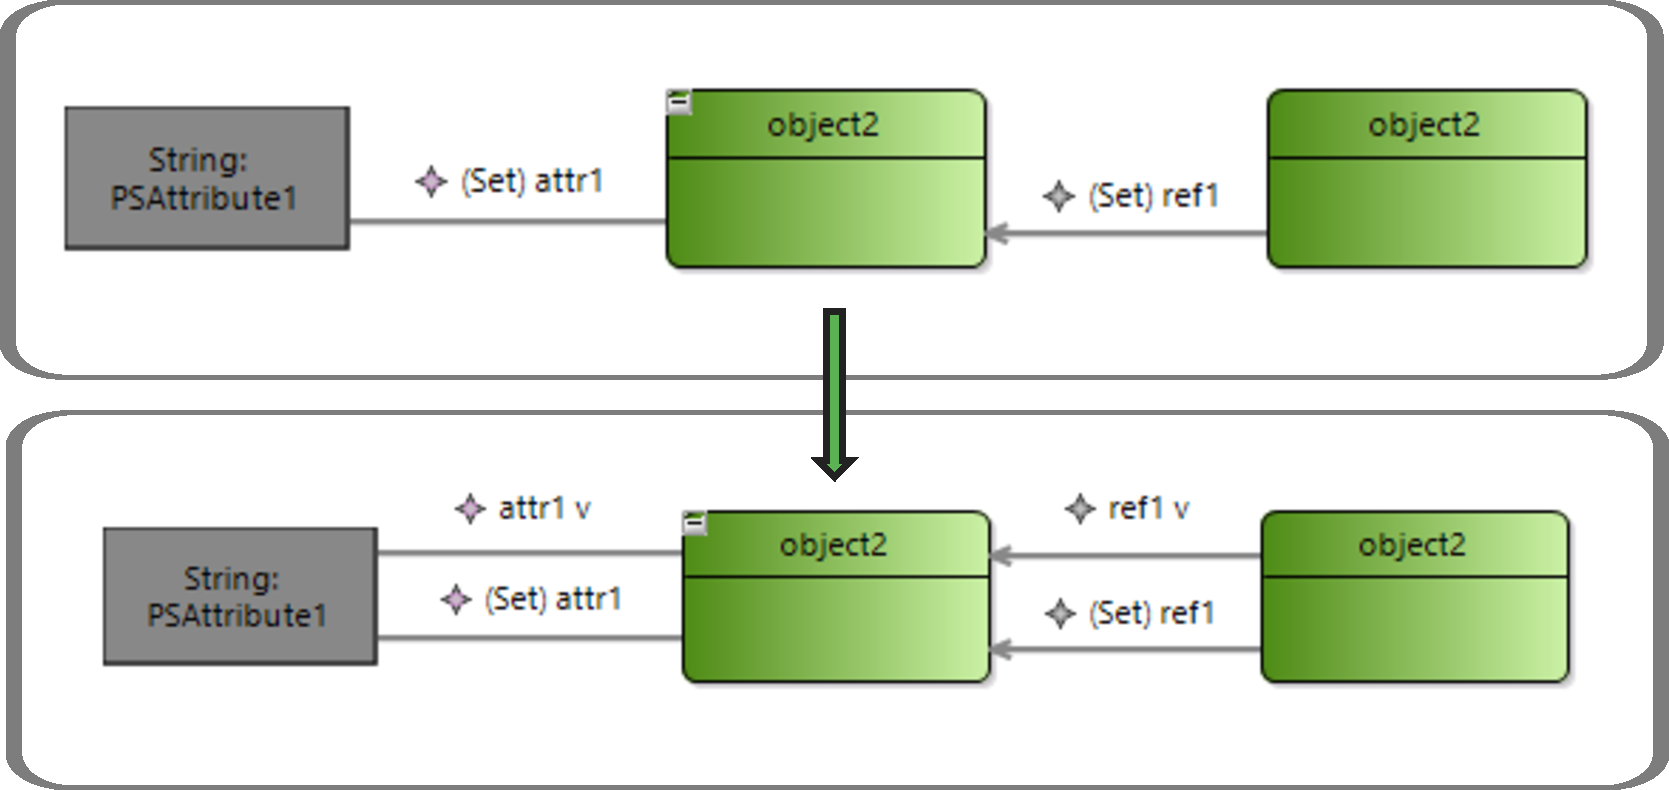
\includegraphics[width=100mm]{figures/refset.pdf}
	\caption{PSReference finomítása (Set)}
	\label{refset} 
\end{figure}

\subsubsection{Var részlegességről általában}
Eredeti objektumnak, elemnek nevezzük azt az PSObject-et amelyiknek a 'Var' részlegességére duplán kattintottunk. A 'Var' részlegességnek van egy id-ja, ami segítségével meg lehet jelölni, hogy melyik 'Var' részlegességek tartoznak egybe, erre a későbbiekben 'Var id'-val hivatkozom.


\subsubsection{PSObject Var feloldása}
 Az összes olyan objektumnak, amelyiknek megegyezik a 'Var id'-ja az törlődik, kivéve az eredeti de előtte az összes hozzá tartozó referencia mintájára létrejönnek az eredeti objektumban élek. Azok az objektumok élei amikből eddig egy törölt objektumba mutattak, azok most az eredeti objektumra fognak mutatni (lásd \autoref{objvar}).
\begin{figure}[!ht]
	\centering
	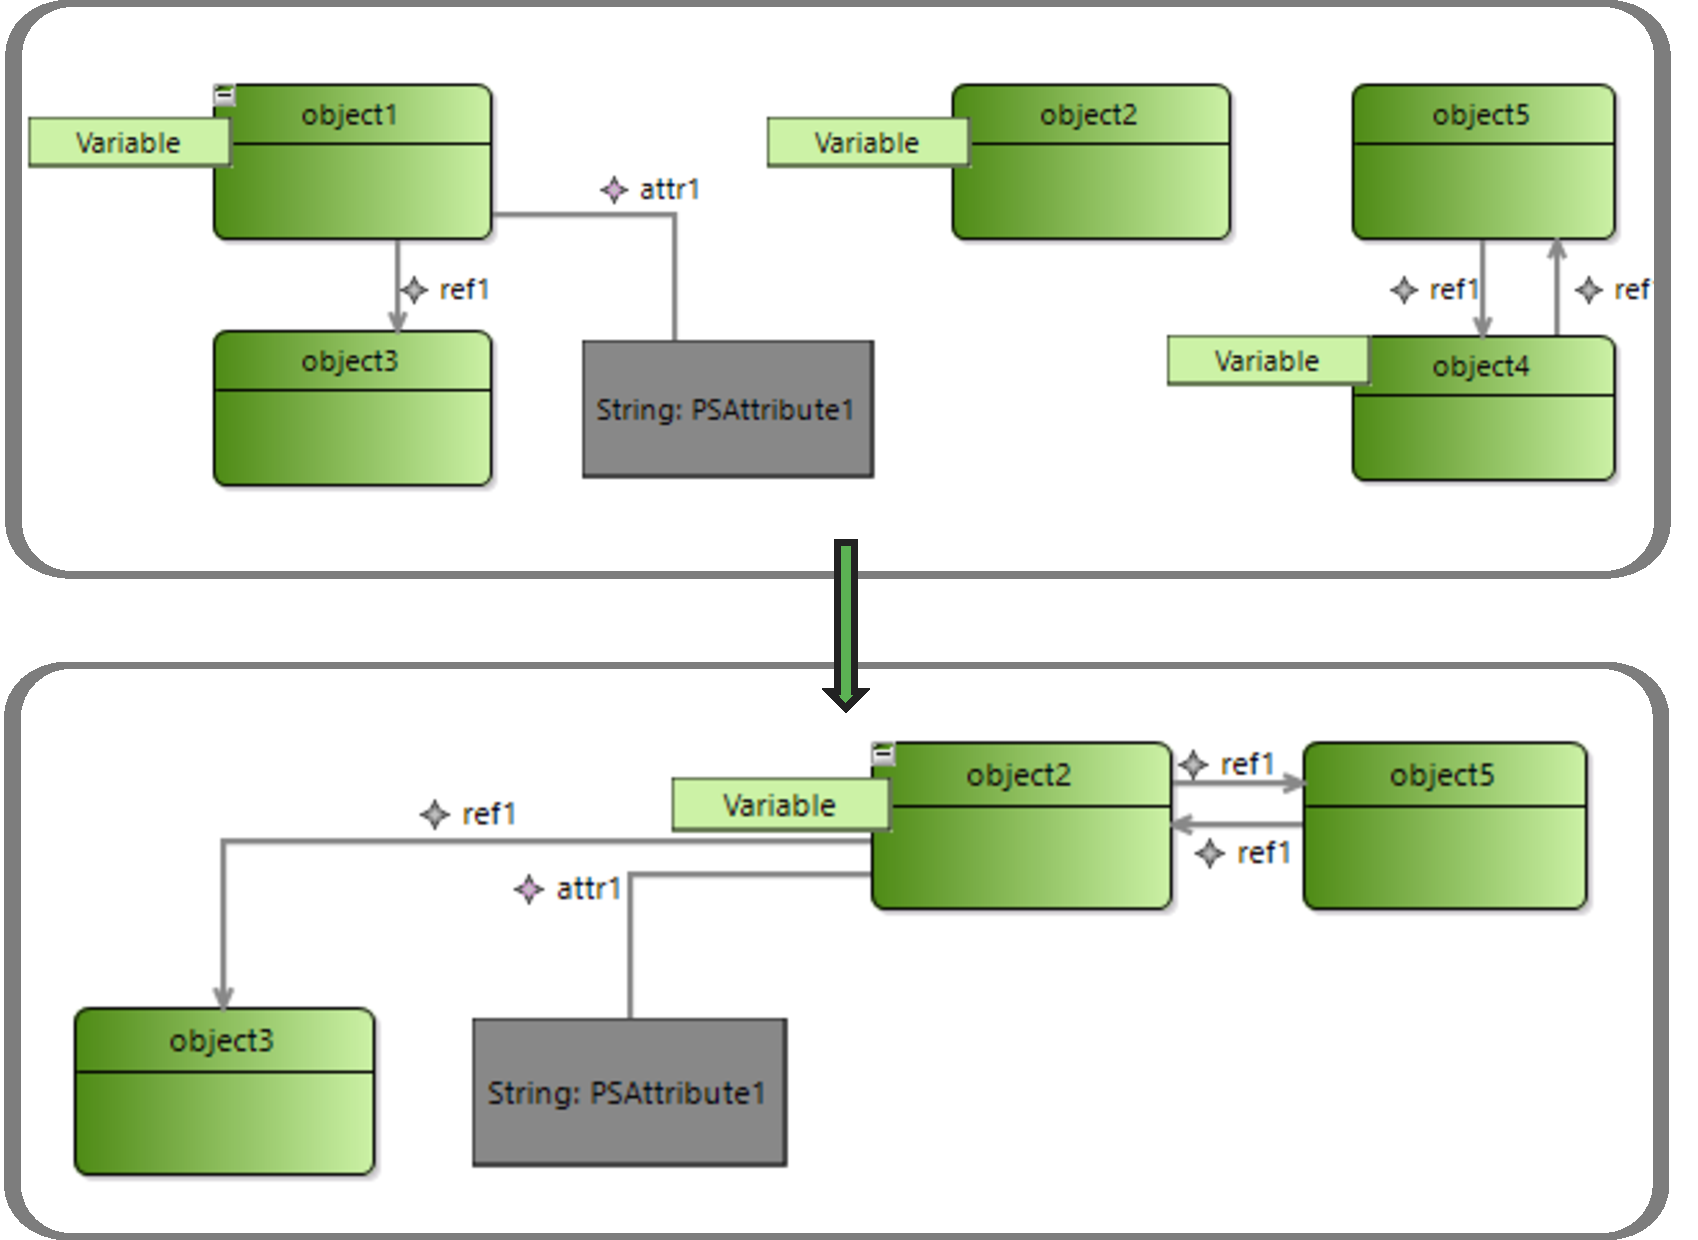
\includegraphics[width=110mm]{figures/objvar.pdf}
	\caption{PSObject finomítása (Var)}
	\label{objvar} 
\end{figure}

\subsubsection{PSAttribute Var feloldása}
Az eredetin kívül az összes olyan attribútum kitörlődik, aminek a 'Var id'-ja megegyezik az eredeti elem 'Var id'-jával. A törölt elemekbe futó élek az eredeti elemre fognak ezentúl mutatni (lásd \autoref{attrvar}).
\begin{figure}[!ht]
	\centering
	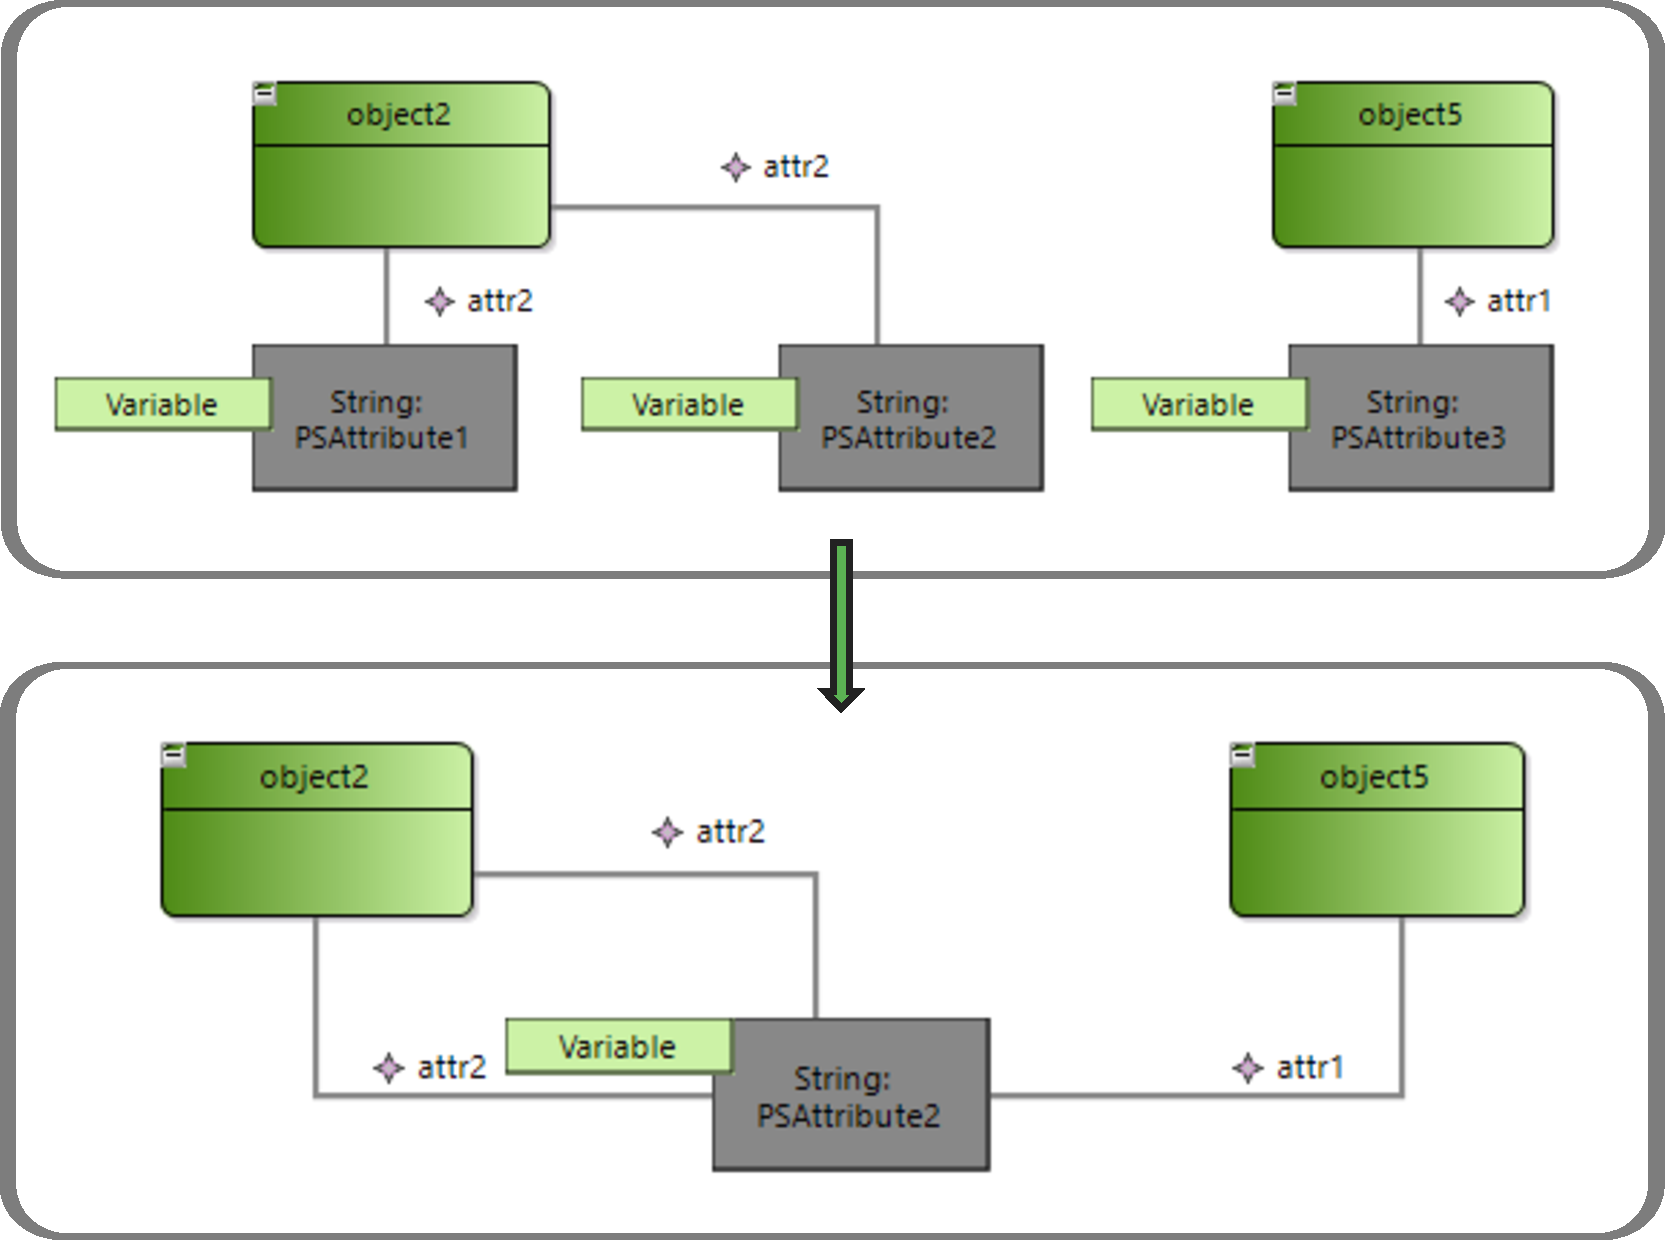
\includegraphics[width=110mm]{figures/attrvar.pdf}
	\caption{PSAttribute finomítása (Var)}
	\label{attrvar} 
\end{figure}

\subsubsection{PSReferenceToObject Var feloldása}
Csak az eredeti referencia forrásobjektumában keres vele megegyező 'Var id'-val rendelkező referenciát. Ezeket a referenciákat törli (lásd \autoref{refvar}).


\subsubsection{PSReferenceToAttribute Var feloldása}
Hasonlóan a PSReferenceToObject esetéhez csak az eredeti referencia forrásobjektumában keres vele megegyező 'Var id'-val rendelkező referenciát. Ezeket a referenciákat törli (lásd \autoref{refvar}).

\begin{figure}[!ht]
	\centering
	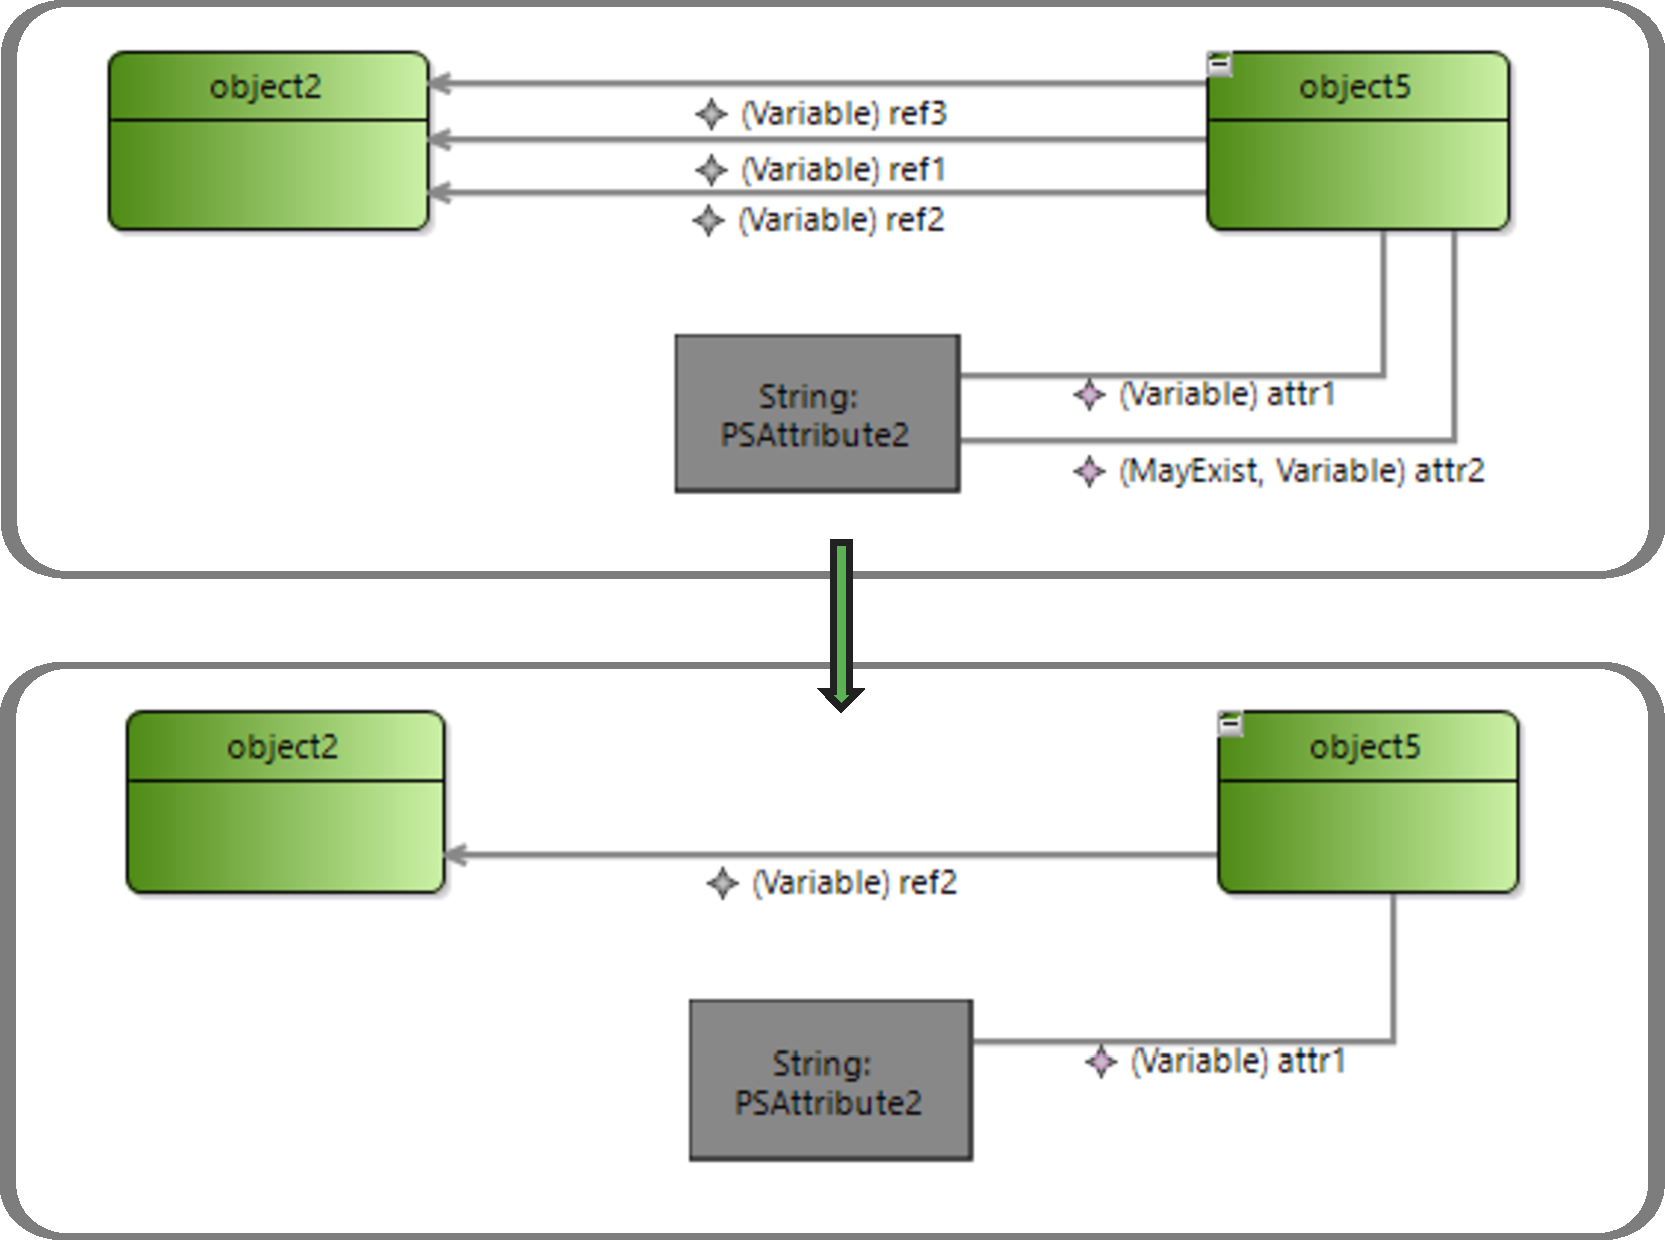
\includegraphics[width=110mm]{figures/refvar.pdf}
	\caption{OSReference finomítása (Var)}
	\label{refvar} 
\end{figure}